\section{Robot Path Planning Based on CSA}
\frame
{
\frametitle{Robot Path Planning Based on CSA}
\framesubtitle{A. Antibody Encoding}
\begin{itemize}
	\item One of the main problem to start solving the problem with CSA.
	\item The encoding depends on the problem.
	\item Robot environment represented by orderly numbered grids.
	\item Boundary of obstacles plus minimum safety distance.
	\item A path is encoded as a sequence of grid numbers.
\end{itemize}
}


\frame
{
\frametitle{Robot Path Planning Based on CSA}
\framesubtitle{A. Antibody Encoding}
\begin{itemize}
	\item In the grid, suppose $(i,j)$ (grid) and $(x,y)$ (environment coordinate). $a$ denotes the side length.
	\begin{eqnarray}
		i &=& int(x/a) + 1 \\
		j &=& int(y/a) + 1 \nonumber\\\nonumber\\ 
		x &=& (i - 0.5)\cdot a \\
		y &=& (j - 0.5)\cdot a \nonumber
	\end{eqnarray}
\end{itemize}
}

\frame
{
\frametitle{Robot Path Planning Based on CSA}
\framesubtitle{A. Antibody Encoding}
\begin{itemize}
	\item A antibody us defined a robot path.
	$$X := {a_{0}, a_{1}, \ldots, a_{n}} $$
	\item $a_{0}$ and $a_{n}$ are fixed numbers (start and end).
	\item $a_{1}, \ldots. a_{n-1}$ are grid numbers.
	\item Two numbers of the antigen cannot be equals.
\end{itemize}
}

\frame
{
\frametitle{Robot Path Planning Based on CSA}
\framesubtitle{A. Antibody Encoding}
\begin{center}
	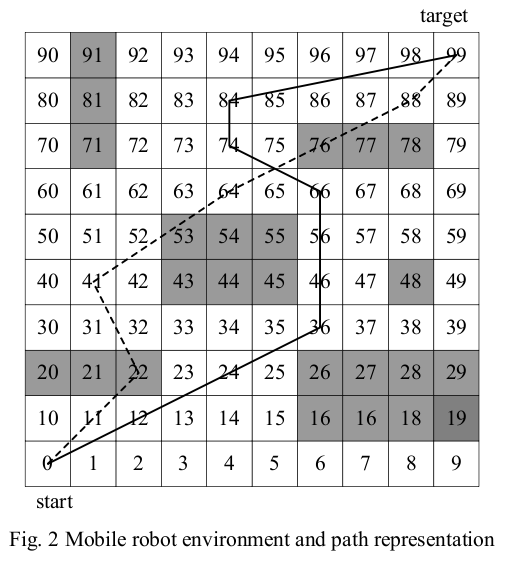
\includegraphics[width=0.5\textwidth]{img/diagram1}
\end{center}
}

\frame
{
\frametitle{Robot Path Planning Based on CSA}
\framesubtitle{B. Fitness Function}
\begin{itemize}
	\item A path can be feasible (collision free) or not.
	\begin{eqnarray}
		fitness &=& \frac{A}{f} \nonumber \\
		f &=& \sum_{i=1}^{N}(d_{i} + C\beta_{i}) \nonumber
	\end{eqnarray}
	\item $A$ is a constant which is decided by the robot environment (A=20).
	\item $f$ is path evaluation function.
	\item $N$ is the number of line segments of a path.
	\item $d_{i}$ is the Euclidean distance of the two nodes forming the line segment (complex compute)
\end{itemize}
}
\frame
{
\frametitle{Robot Path Planning Based on CSA}
\framesubtitle{B. Fitness Function}
\begin{itemize}
	\item $C$ is a constant.
	\item $\beta_{i}$ is the coefficient denoting depth of collision:
	\[
	\beta_{i} = \left\{ 
		\begin{array}{l l}
	    0                         & \quad \text{if the $i$th line do not intersect with obstacle(s)}\\
	    \sum_{j=1}^{M} \alpha_{j} & \quad \text{if the $i$th line intersects with obstacle(s) }\\
		\end{array} \right.
	\]
	\begin{itemize}
		\item $M$ is the number of obstacles the line segment intersects.
		\item $\alpha_{j}$ is determined by considering how deep a line segment intersecs an obstacle $j$. 
	\end{itemize}
\end{itemize}
}

\frame
{
\frametitle{Robot Path Planning Based on CSA}
\framesubtitle{C. Selection Strategy}
\begin{itemize}
	\item Is an important problem, because is the preconditioning of Clonal and Hyper-mutation.
	\item Many methods how to select these individuals:
	\begin{itemize}
		\item Roulette wheel.
		\item Boltzman selection.
		\item Tournament selection.
		\item Rank selection.
		\item Steady state selection
		\item etc.
	\end{itemize}
	\item In this paper the winner is \textbf{Roulette Wheel}.
\end{itemize}
}

\frame
{
\frametitle{Robot Path Planning Based on CSA}
\framesubtitle{D. Immune operators}
\begin{itemize}
	\item Many operators from GA can be user in CSA.
	\item Three immune operators are devised for the path planning. 
\end{itemize}
}

\frame
{
\frametitle{Robot Path Planning Based on CSA}
\framesubtitle{D. Immune operators}
\begin{itemize}
	\item Mutation Operator:
	\begin{itemize}
		\item Randomly chooses a node and replaces it with a node that is not included in the path.
		\item In CSA is very different to GA.
		\begin{itemize}
			\item In GA, fitness value of individual is proportional to mutation rate (in CSA is inverse)
		\end{itemize}
		\item Served as role to accelerate convergence (hyper-mutation), meanwhile in GA is served to diversify the solution population.
	\end{itemize}

	\begin{center}
		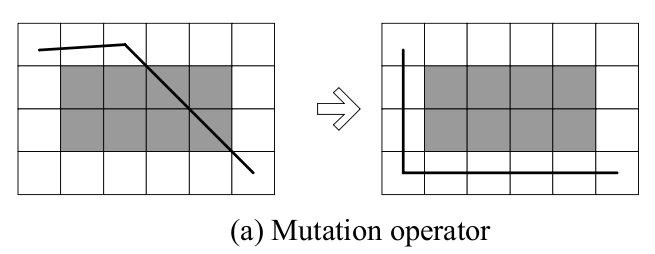
\includegraphics[width=0.6\textwidth]{img/mutation}
	\end{center}
\end{itemize}
}

\frame
{
\frametitle{Robot Path Planning Based on CSA}
\framesubtitle{D. Immune operators}
\begin{itemize}
	\item Insertion Operator:
	\begin{itemize}
		\item Used to repair an infeasible line segment, inserting a suitable node between.
		\item To locate the best node, is applied a similar local search in the all of neighboring grids of the intersected obstacle.
	\end{itemize}
	\begin{center}
		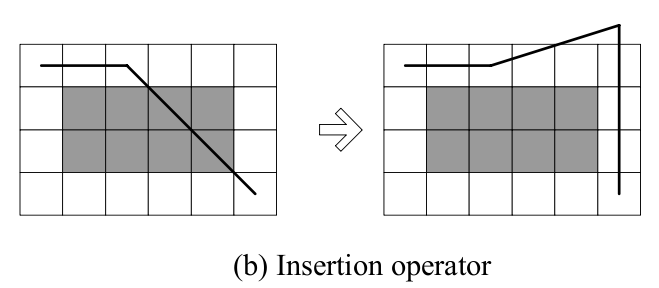
\includegraphics[width=0.6\textwidth]{img/insertion}
	\end{center}
\end{itemize}
}

\frame
{
\frametitle{Robot Path Planning Based on CSA}
\framesubtitle{D. Immune operators}
\begin{itemize}
	\item Deletion Operator:
	\begin{itemize}
		\item Is applied to feasible and infeasible path.
		\item Randomly choose one node, check its two adjacent nodes, and connected segments.
		\item If this produce a beneficial action, delete node.
	\end{itemize}
	\begin{center}
		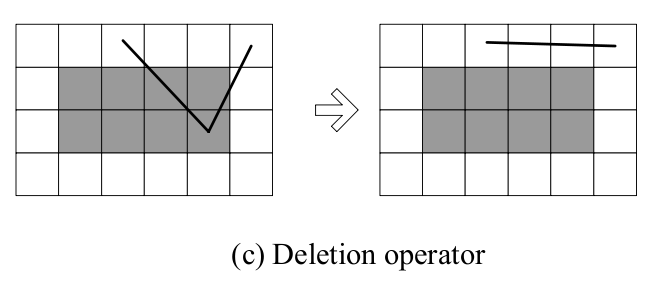
\includegraphics[width=0.6\textwidth]{img/deletion}
	\end{center}
\end{itemize}
}

\frame
{
\frametitle{Robot Path Planning Based on CSA}
\framesubtitle{E. CSA based Flow Chart of Mobile Robot Path Planning}
\begin{enumerate}
	\item Initializing parameters. (probabilities, max sizes, etc.)
	\item Creating population including $n$ paths randomly.
	\item Evaluate fitness.
	\item Immune selection.
	\item Clone operation.
	\item Hyper-mutation.
	\item Create some new antibody.
	\item Insertion and deletion operators.
\end{enumerate}
}

\frame
{
\frametitle{Robot Path Planning Based on CSA}
\framesubtitle{E. CSA based Flow Chart of Mobile Robot Path Planning}
\begin{center}
	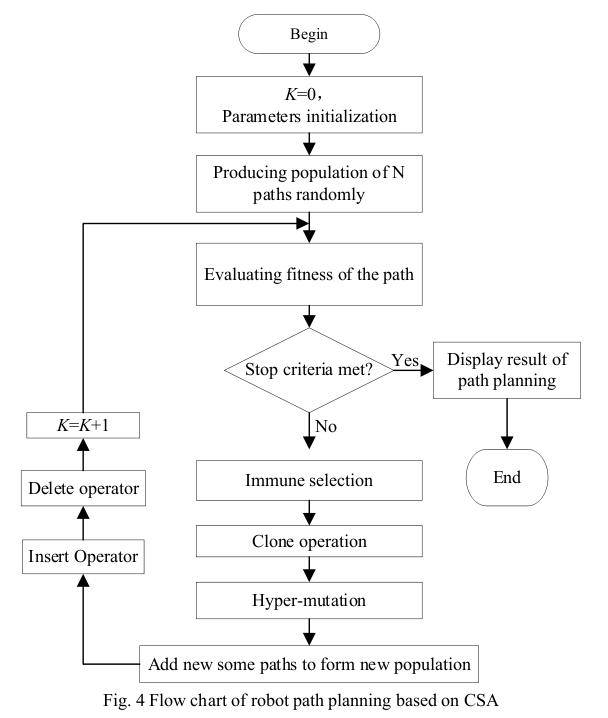
\includegraphics[width=0.5\textwidth]{img/diagram2}
\end{center}
}
